% gold_figures_memo.tex
%
% A memo built around the four finished figures in ./figures/. Six to seven
% pages, declarative section headings, endnotes.
%
% The four figures arrive here already rendered; nothing in this folder draws
% them. Every number in the prose is recomputed from the raw pulls by
% stats/memo_stats.py, whose output is stats/memo_stats.txt. Three quantities
% come from elsewhere and say so where they appear: the daily curve-fit
% diagnostics (gold_final/data/fig2.log), the transfer-cost build-up and the
% episode's resource bill (gold_final/letter/gold_letter.tex).
%
% This covers the same ground as gold_final/memo/gold_memo.tex, which was
% written against the earlier Stata renderings. Where the two differ in a
% number, this one is the later and the reason is given in the folder README.
%
% NOT a Federal Reserve publication and deliberately not dressed as one.
%
% Build (two passes, for the endnote numbering):
%   pdflatex -interaction=nonstopmode gold_figures_memo.tex
%   pdflatex -interaction=nonstopmode gold_figures_memo.tex

\documentclass[11pt]{article}

\usepackage[letterpaper,margin=1.0in,top=0.95in,bottom=1.0in]{geometry}
\usepackage[T1]{fontenc}
\usepackage[utf8]{inputenc}
\usepackage{charter}
\usepackage[scaled=0.92]{helvet}
\usepackage{graphicx}
\usepackage{amsmath}
\usepackage{booktabs}
\usepackage{enumitem}
\usepackage{endnotes}
\usepackage{caption}
\usepackage{microtype}
\usepackage[hidelinks]{hyperref}
\usepackage{xcolor}

\definecolor{ink}{HTML}{121212}
\definecolor{soft}{HTML}{555555}
\definecolor{rule}{HTML}{BBBBBB}

\usepackage{titlesec}
\titleformat{\section}{\sffamily\bfseries\large\color{ink}}{}{0pt}{}
\titlespacing*{\section}{0pt}{14pt}{5pt}

\captionsetup[figure]{labelformat=empty, justification=raggedright,
  singlelinecheck=false, font={sf,small}, skip=6pt}

% Let a figure share a page with text instead of claiming one to itself. The
% defaults reserve 20% of every float page for nothing, which with four
% full-width figures costs the better part of a page.
\renewcommand{\topfraction}{0.92}
\renewcommand{\bottomfraction}{0.75}
\renewcommand{\textfraction}{0.06}
\renewcommand{\floatpagefraction}{0.80}

\setlength{\parskip}{5pt}
\setlength{\parindent}{0pt}
\renewcommand{\baselinestretch}{1.03}

\renewcommand{\enotesize}{\footnotesize}
\renewcommand\enoteheading{\section*{\sffamily\bfseries\large Notes}}

% \raggedright is needed because the figure environment centres everything,
% which left the notes block centred line by line.
\newcommand{\fignote}[2]{%
  \par\vspace{2pt}{\raggedright\sffamily\scriptsize\color{soft}%
  \textbf{Notes:} #1\par\textbf{Sources:} #2\par}}

\begin{document}
\pagestyle{empty}

% ------------------------------------------------------------------ masthead
{\sffamily\footnotesize\color{soft} ECONOMIC RESEARCH MEMO \hfill October 2026}

\vspace{4pt}
{\color{rule}\hrule height 2pt}
\vspace{10pt}

{\sffamily\bfseries\LARGE\color{ink}
Financial gold and the trade accounts:\\ why the ITA needs a bullion adjustment\par}

\vspace{6pt}
{\sffamily\small\color{soft} Samuel Moore\par}

\vspace{10pt}

% ------------------------------------------------------------------ abstract
{\sffamily\small\color{ink}
In January 2025 the United States imported 393 tonnes of gold in a single
month, thirty times what Americans buy as jewellery and retail investment in a
month. The inflow peaked that March; eleven months later all of it had gone
back out. This memo argues that
these flows were financial rather than commercial, that the structure of the
gold market is what makes them so, and that their passage through the
International Transactions Accounts left two official measures of the U.S.\
goods balance pointing in opposite directions for three consecutive quarters.
Published GDP is unaffected: the national accounts already remove nonmonetary
gold. The monthly trade release does not --- and the adjustment that fixes it
is arithmetic on published data, verifiable against the national accounts, and
safe to apply as the occasion demands.\par}

\vspace{6pt}
{\color{rule}\hrule height 0.5pt}

% ====================================================================
\section{An outlier among traded goods}

Between November 2024 and March 2025, one line of the U.S.\ trade accounts did
something the rest of them never do. Gold imports, which ran between \$0.6 and
\$2.6 billion a month across 2015--2019, reached \$34.2 billion in January 2025
alone --- 10.5\% of all U.S.\ goods imports in a single month, from a commodity
that averaged 0.55\% of them over those five earlier years. It had happened
once before, smaller: gold reached 7.2\% and 8.8\% of goods imports in April
and May 2020.

Then it reversed. Figure 1 places gold against the hundred most-traded U.S.\
commodity headings on the balance plane --- exports on one axis, imports on the
other, averaged within three phases, on log scales. Above the diagonal the
United States is a net importer of a good; below it, a net exporter. Most
commodities sit still, their three phase points nearly on top of one another,
which is what a traded good looks like over two years. Gold travels almost
straight up into the surge, as monthly imports go from \$1.95 billion to
\$19.41 billion with exports barely moving, and then down and to the right into
the reversal, as exports go from \$3.40 billion to \$10.87 billion a month. It
ends as far below the diagonal as it began above it.

\begin{figure}[htbp]
\centering
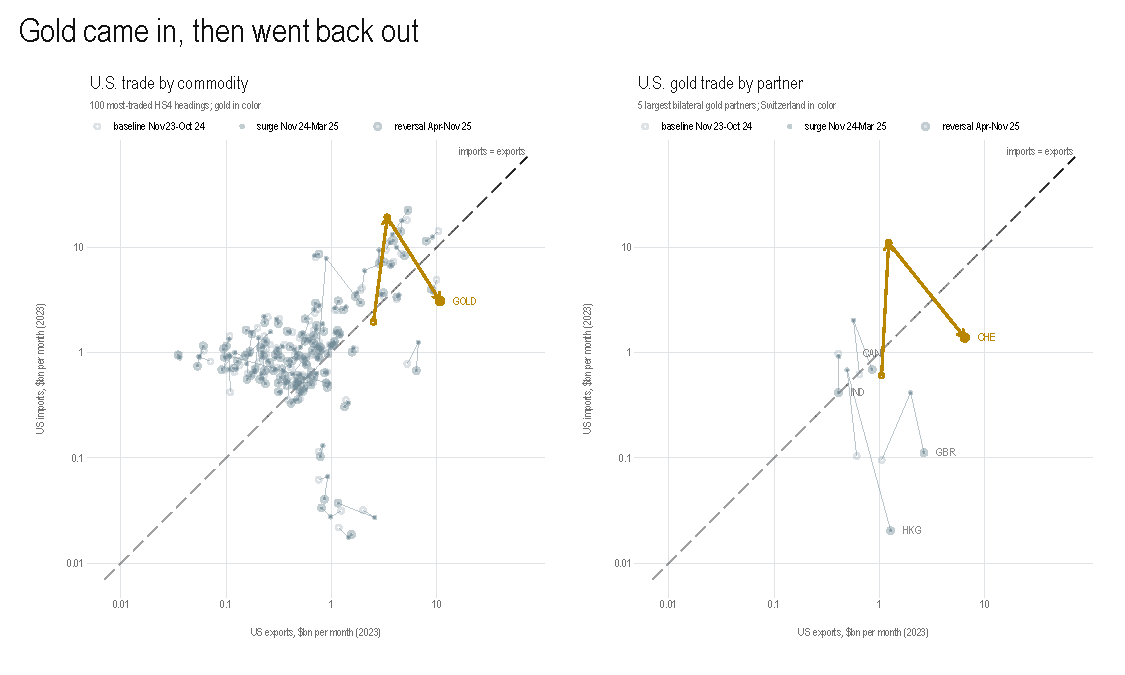
\includegraphics[width=0.96\textwidth]{figures/combo.pdf}
\caption{\textbf{1. Gold's round trip, against every other traded good}}
\fignote{Monthly averages within each phase, log scales on both axes, so a
point's distance from the diagonal is the ratio of imports to exports, not
their difference. Partner panel: the regional aggregates Census returns on the
same endpoint are excluded, so the five are countries.}{U.S.\ Census Bureau,
monthly HS4 trade.}
\end{figure}

The right-hand panel names the partner that carried most of it. Switzerland
takes 27\% of identified U.S.\ gold imports in the baseline and 57\% during the
surge, then supplies 57\% of identified exports in the reversal --- the same
excursion, in one bilateral relationship. The other four trace much shorter
paths.

The round trip is the first evidence that this was not trade in the ordinary
sense. Cumulative net gold imports ran to \$80.0 billion by March 2025, crossed
back through zero in February 2026, and stood at \$47.6 billion \emph{negative}
by July 2026: more metal left than had arrived.\endnote{Cumulated from November
2024, the surge's first month. Over the whole window since 2015 net flows are
\$64 billion negative, so the direction is the same on a longer reckoning.}
Across that whole window, \$791 billion of gold crossed the U.S.\ border gross
against a net of \$-64 billion. Ninety-two percent of the recorded trade was
metal going one way and coming back.

Goods that are bought get consumed, installed or worn. They do not come back.

% ====================================================================
\section{Nobody at either end wanted the metal}

A sceptical reader can still ask whether Americans were simply buying a lot of
gold, and foreigners buying it back. The answer is arithmetic, and Figure 2
gives it on both sides of the account, month by month.\endnote{Census reports value and not mass for HS 7108 and 7115, so every
tonnage here is \emph{derived} --- the month's customs value over the LBMA PM
monthly mean, at 32,150.7 troy ounces to the tonne --- rather than reported. It
is a different measurement of the same flow from the mass in the Swiss and
British returns and will not agree to the tonne.}

The upper panel sets U.S.\ gold imports against U.S.\ demand: jewellery plus
bar and coin, which is every ounce Americans buy as ornament or hold as retail
investment. The benchmark is deliberately generous: bar and coin is investment
rather than fabrication, and including it makes the comparison harder to
win.\endnote{Technology demand --- electronics, dental, industrial --- would add
little. It runs near 330 tonnes a year for the entire world, and the World Gold
Council does not publish it by country.} U.S.\ demand is the flattest line in
this memo. It has averaged 16.6 tonnes a month since 2015 and has never
exceeded 27.7 in any month or 83 in any quarter. January 2025 brought in 393
tonnes against 13.0 tonnes of demand --- thirty times a month's consumption, in
one month. Over the five surge months the ratio is thirteen to one.

\begin{figure}[htbp]
\centering
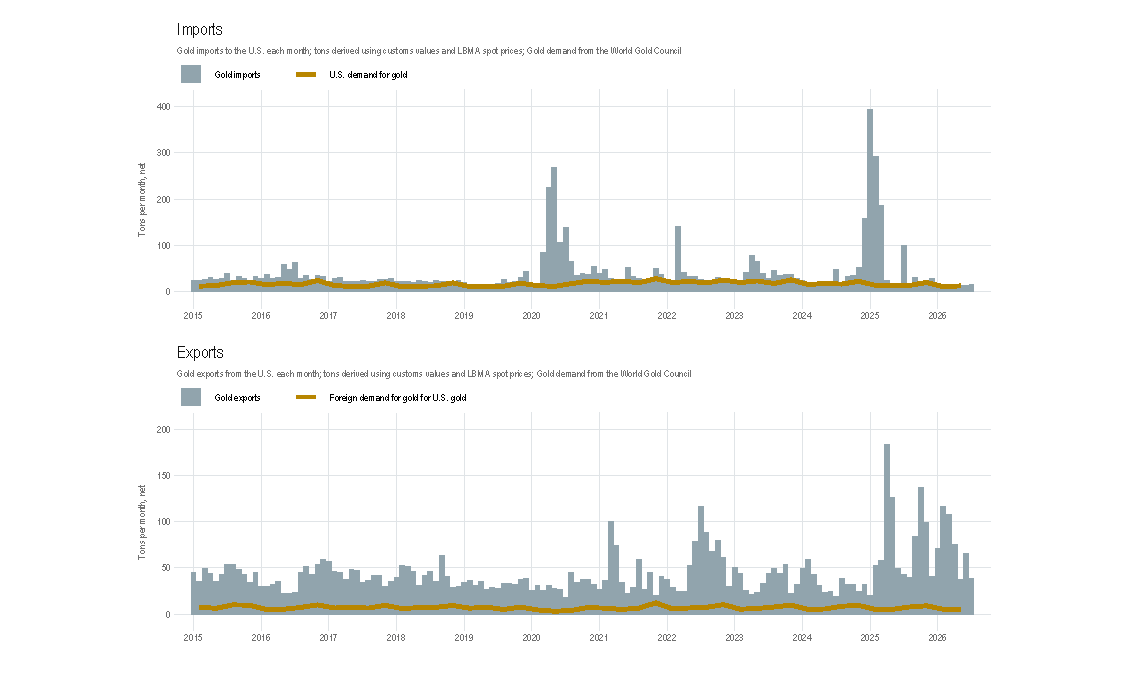
\includegraphics[width=0.89\textwidth]{figures/demand_combo.pdf}
\caption{\textbf{2. The flows against what the metal is actually used for}}
\fignote{Tonnes a month, derived from Census customs values at the LBMA PM
monthly mean. Demand is jewellery plus bar and coin, scaled in the lower panel
by the U.S.-supplied share of each destination's gold imports. The five
destinations are read off the trade data, not assumed, and their membership is
not stable: Canada is fifth on a window beginning in 2022. The World Gold
Council does not break out Swiss jewellery demand, which sits inside a regional
aggregate, so Switzerland contributes bar and coin only and the benchmark is
marginally understated.}{U.S.\ Census Bureau; UN Comtrade; HMRC; Swiss Federal
Office for Customs and Border Security; World Gold Council, \textit{Gold Demand
Trends}; LBMA.}
\end{figure}

The lower panel does the same for exports, against the demand of the five
destinations that take them --- Hong Kong, India, Singapore, Switzerland and
the United Kingdom, together 86.5\% of U.S.\ gold exports to identified
countries. All five buy gold from many suppliers, so setting U.S.\ exports
against their \emph{entire} demand would overstate what the United States could
plausibly be supplying. Each destination's demand is therefore scaled by the
share of its gold imports the United States provides --- in every case the
largest figure any source reports in any year, which makes the benchmark larger
and this comparison harder to win.\endnote{United Kingdom 26\%, Switzerland
25\%, Hong Kong and Singapore 12\%, India 10\%: each the maximum across UN
Comtrade on both a mass and a value basis and, where an independent national
compiler exists, HMRC (24.5\%), the Swiss customs administration (17.7\%) and
Metals Focus via the World Gold Council (6.3\%). Applying one year's peak flat
across eleven years is generous again on top of taking the maximum.} So scaled, the five's
reachable demand averages 7.9 tonnes a month, against total U.S.\ gold exports
averaging 45. April 2025 shipped 183 tonnes, thirty-one times that month's
benchmark, and exports clear it in all 139 months of the window --- 6,262
tonnes out against 1,094 tonnes that could have been absorbed.

The composition cuts against the argument before it cuts for it. India is in the
set and is a genuine consumption market --- more jewellery and retail bar than
the other four together --- and at its 10\% share it supplies 6.0 of the
benchmark's 7.9 tonnes a month, so three-quarters of the lower panel's line is
India. Yet India takes only 5.7\% of the tonnage shipped to the five, while
Switzerland and the United Kingdom take 79\% and account for 1.5 tonnes a month
of demand between them. The metal goes to the refineries and the vaults, not to
where the jewellery is made.

So something moved 393 tonnes in a month that nobody at either end had any use
for, and then moved most of it back. What?

% ====================================================================
\section{Two prices for the same metal}

Gold trades in two places that are not quite the same market. London is an
over-the-counter market in 400-ounce \textit{Good Delivery} bars, held
unallocated in vaults and settled by book entry. New York is a futures
exchange, COMEX, whose contract delivers 100-ounce bars into registered
exchange warehouses. The metal is identical. The venue, the bar, and the legal
form of the claim are not.

Because the two can be converted into each other, arbitrage ties their prices
together --- but only loosely, and the slack is the subject of Figure 3. The
futures price should exceed the spot price by the cost of carrying metal to
delivery: financing plus storage. That is the same no-arbitrage logic as
covered interest parity, with a storage cost in place of a foreign interest
rate. The upper panel plots the estimated COMEX--London spread at a fixed
ninety-day horizon against exactly that carry cost.\endnote{The spread is the
intercept of a daily open-interest-weighted projection of the whole futures
curve onto days-to-delivery, corrected for the three and a half hours between
the COMEX settlement and the London benchmark. That correction is not cosmetic:
across 2,862 days in the fit, 2,851 of them re-timed, it cuts the standard
deviation of the premium from 0.499\% to 0.235\%. Fitting the curve rather than
differencing a single contract keeps the delivery calendar out of the series; at
4.5\% financing on \$4,400 gold the roll alone generates a sawtooth of roughly
\$33 an ounce, comparable to the dislocations being hunted.}

\begin{figure}[htbp]
\centering
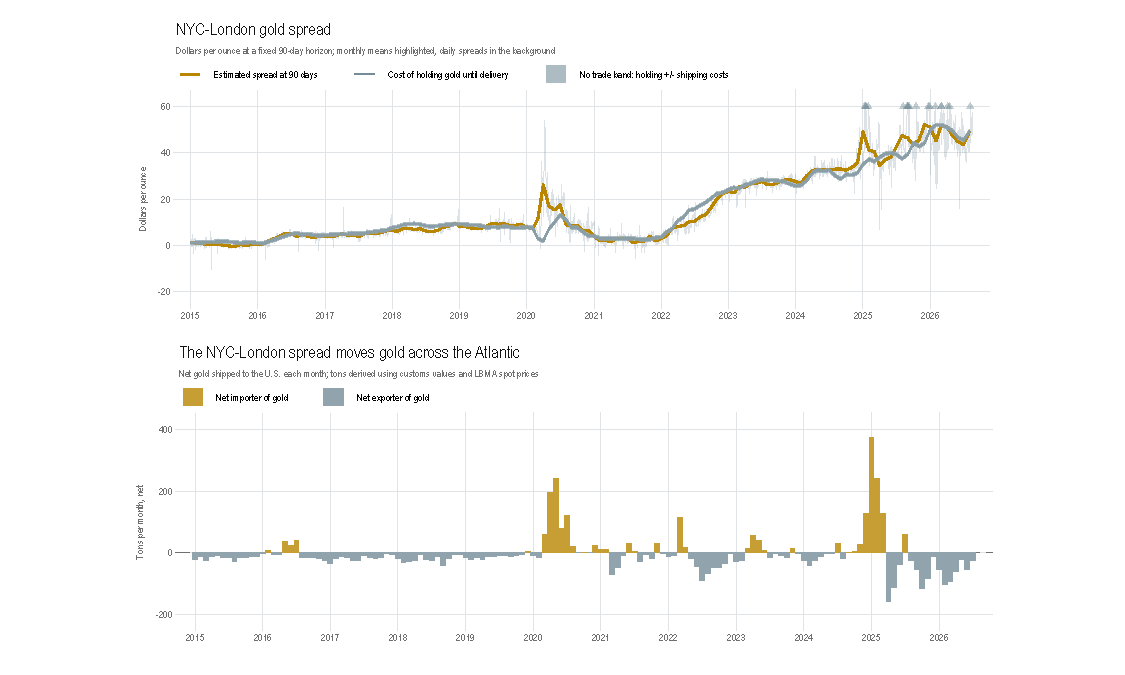
\includegraphics[width=0.89\textwidth]{figures/spread_combo.pdf}
\caption{\textbf{3. The spread against what it has to clear, and the metal that
followed}}
\fignote{Upper panel: daily spreads in grey behind monthly means. Daily
observations outside the axis are marked at the top rather than dropped. The
no-trade band is carry plus and minus an all-in transfer cost of \$0.75 an
ounce --- \$0.35 of published COMEX depository delivery-out charge, \$0.20 of
air freight and \$0.20 of recasting. Lower panel: net derived tonnage, both
headings, gold where the United States was a net importer that month.}{CME via
Databento, GLBX.MDP3, re-timed to the LBMA auction; LBMA; U.S.\ Census Bureau.}
\end{figure}

The first thing the panel shows is how much of the dollar spread is not a
dislocation at all. The two lines rise together from about a dollar an ounce in
2015 to the mid-forties by 2026, and almost all of that is carry: higher policy
rates and a higher gold price make the same financing cost a bigger number. A
reader watching the raw spread quadruple would conclude the market was
dislocating when mostly money had become expensive. The question is never the
spread's level; it is the gap between the spread and the line beneath it.

The second is that the gap has to be large enough to pay for moving metal.
Freight and insurance, the exchange's delivery-out charge and recasting come to
roughly \$0.75 an ounce each way, and that is the width of the shaded band.
Below it nothing moves in either direction: the relationship is a threshold,
not a slope. Across the fit, 851 days clear the band to the west and 1,287 to
the east, so both regimes are well represented and any specification has to
handle both.\endnote{Sign is directional. Above the band New York is rich and
metal flows west; below it New York is cheap and metal flows east. The \$0.75
figure is built up from a published tariff and two reported institutional
rates, not from quotes we obtained; a single carrier quote would be the
cheapest available improvement to this figure.}

The lower panel is what followed. Of 139 months, 105 are net eastward: the
United States is normally a net exporter of gold, which is the first thing most
readers of the 2025 headlines did not know. The exceptions line up with the
exceptions above --- 2020 and, far larger, the winter of 2024--25, when the
spread sat clear of the band for months and 867 tonnes moved west between
December and March. From April to August 2025, with the band cleared the other
way, 281 tonnes went back.

One further feature of the market matters for what the trade statistics record.
London bars and COMEX bars are different sizes, so relocating metal between the
two generally requires recasting, and the refining capacity sits mostly in
Switzerland. A single tonne moved from London to New York can therefore be
recorded as several crossings --- out of the United Kingdom, into Switzerland,
out of Switzerland, into the United States. The gross trade footprint of a
relocation substantially exceeds the relocation itself, which is why
Switzerland dominates the partner panel of Figure 1. It also explains why the
episode was so cheap in real resources: counting a round trip as two flights
and two recastings gives 1,632 tonne-legs and a bill near \$243 million, range
\$85 million to \$520 million, against \$174 billion of metal carried ---
0.14\% of the value moved.\endnote{The wide range reflects insurance and
transit financing, which scale with the gold price and roughly doubled over
this sample. Retail parcel rates of \$300--500 a kilogram are not used here:
they price a one-kilo consignment to a private buyer, not a tonne moving
between bullion banks, and are two orders of magnitude too high.}
Relocating gold is close to free relative to what gold is worth, which is
precisely why a few dollars an ounce of differential could move a quarter of a
year's mine output in five months.

What the spread cannot do is isolate location risk. Four things sit inside it
--- time, place, form and trust --- and carry removes only the first. The
residual plotted here is the sum of the other three, not location risk alone.

% ====================================================================
\section{What it did to the trade accounts}

The Bureau of Economic Analysis publishes the U.S.\ goods balance twice. The
International Transactions Accounts, which underlie the monthly trade release,
count nonmonetary gold as a good --- correctly, under the international
standard.\endnote{BPM6 classifies nonmonetary gold as a good and monetary gold
as a financial asset, so the ITA treatment is not an error. Monetary gold ---
central bank reserve transactions --- is invisible in trade data by the same
convention.} The national accounts
remove it outright, replacing it with domestic production less industrial use.
In ordinary times the two barely differ and no one needs to know which they are
reading.

\begin{figure}[htbp]
\centering
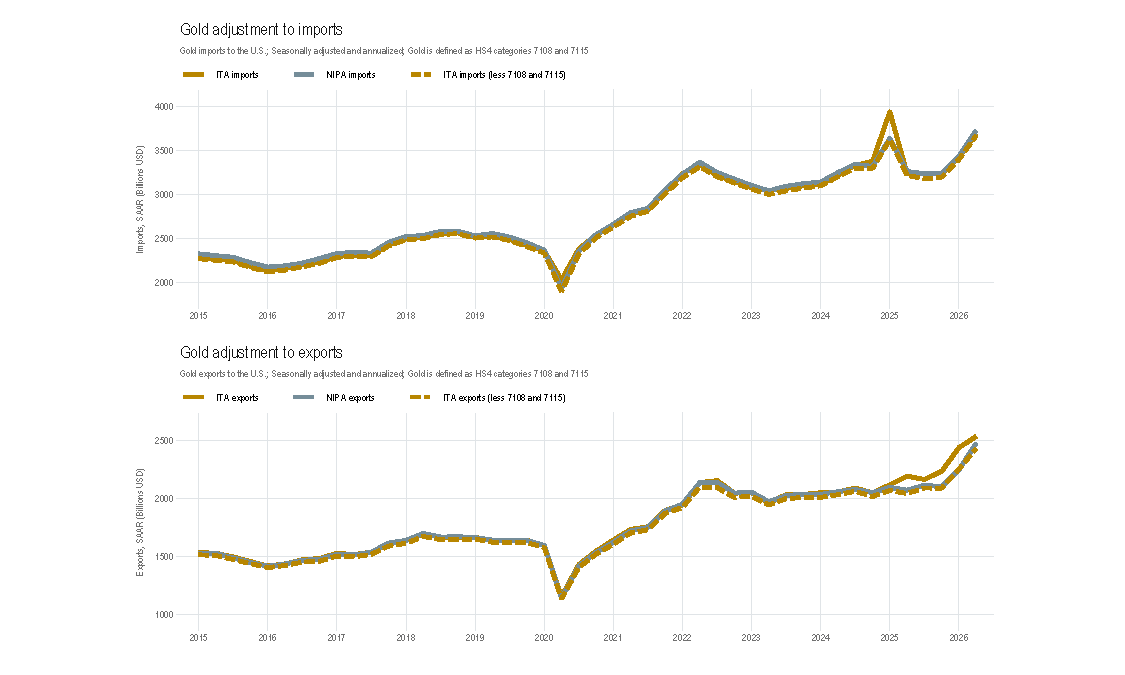
\includegraphics[width=0.89\textwidth]{figures/NIPA_ITA.pdf}
\caption{\textbf{4. The same quarter's trade, measured twice}}
\fignote{Quarterly, at annual rates. ITA monthly figures are averaged over the
months present and multiplied by twelve, so a short quarter is not understated;
the NIPA series are already at annual rates. The adjusted line removes
nonmonetary gold (HS 7108 and 7115) from each side separately. The flows are
shown apart rather than netted because an import error and an export error of
the same sign cancel in a balance, which is what this figure exists to rule out.
The balance statistics in the text come from these same series.}{Bureau of
Economic Analysis, International Transactions Accounts and NIPA table 1.1.5;
U.S.\ Census Bureau.}
\end{figure}

Figure 4 shows what happened when gold stopped being ordinary. On imports the
two series are indistinguishable for ten years and then separate by \$328
billion at an annual rate in 2025Q1 --- the ITA at \$3,967 billion against the
national accounts' \$3,639 billion. On exports the same thing happens a year
later and the other way round, a \$202 billion separation in 2026Q1 as the
metal went home. The gap on each side correlates 0.99 with that side's gold
flow.

In the balance the two effects compound rather than cancel. The 2025Q1 ITA
goods deficit was \$1,826 billion at an annual rate against the national
accounts' \$1,541 billion: a gap of 18.5\% of the latter. Four quarters later
it had swung to \textit{minus} 15.6\%. Across the window the gap correlates
0.98 with net gold trade.

A level gap can be netted out by anyone who knows it is there. A disagreement
about direction cannot, and that is what happened next. In the forty-five
quarterly changes since 2015 the two measures disagree about whether the
deficit widened or narrowed five times. Two are old and isolated, in 2016Q2 and
2018Q4. The other three are recent and consecutive: in 2025Q3 the trade release
showed the deficit widening by \$55 billion while the national accounts showed
it narrowing by \$71 billion, and the next two quarters reversed that. For three quarters running, one official U.S.\ measure of the
external position said it was improving while the other said it was
deteriorating.

The claim is not that either series is wrong; each treatment is correct for its
own purpose. It is that a correct series stopped being informative about what
its readers use it for, and did so without warning them.

% ====================================================================
\section{Adjust it yourself, and check your work}

The practical conclusion is modest: when gold is moving, take it out of the
monthly trade balance before reading anything into the number. The adjustment
is arithmetic, the inputs are published, and --- unusually for an ad-hoc
correction --- you can check that you did it right.

The arithmetic is one line. Because the balance is imports less exports, taking
nonmonetary gold out of both sides is the same as subtracting net gold:
\[
  \text{balance}^{\text{adj}}_{t}
  \;=\;
  \text{balance}_{t} - \bigl(\text{gold imports}_{t} - \text{gold exports}_{t}\bigr).
\]
Both terms come from the Census monthly HS series, under headings 7108 and
7115.\endnote{HS 7108 is unwrought and semi-manufactured gold; 7115 covers
articles of precious metal, under which much of the 2025 inflow was entered.
7108 alone misses most of the episode.} On the headline
goods-and-services balance it reads as follows: January 2025's reported \$124.7
billion deficit becomes \$92.2 billion without the gold, October 2025's
reported \$37.4 billion becomes \$52.6 billion, and the rolling twelve-month
deficit was overstated by \$79.5 billion at its March 2025 peak.

What makes this safe rather than merely convenient is that it can be checked.
The dashed line in each panel of Figure 4 is exactly that calculation, and it
tracks the national accounts. The standard deviation of the import gap falls
from \$53.8 billion to \$9.5 billion and of the export gap from \$38.6 billion
to \$6.6 billion; on the balance the mean absolute gap falls from \$36 billion
to \$11 billion, the 2025Q1 discrepancy from \$285 billion to \$17 billion, the
correlation of quarterly changes rises from 0.908 to 0.991, and all three of
the consecutive directional disagreements vanish. The adjusted series does not
merely look tidier --- it reproduces an independently constructed official
aggregate, built to a different standard by a different part of the same
agency. An ad-hoc correction with an external benchmark is not really ad hoc;
it is a replication.

Three things it does not do, and the figure shows all three. It does not land on
the national accounts in \emph{level}: the dashed line sits about \$18 billion
below NIPA imports and \$9 billion below NIPA exports on average, because
removing all of 7108 and 7115 takes out slightly more than the national accounts
net out, which add back domestic production less industrial use. The claim is
co-movement, not level, and a stable offset is one a reader can carry. It leaves
the two pre-2020 disagreements untouched, as it should --- they are not gold's
doing. And in 2016Q3 it \emph{creates} one: the deficit barely moved that
quarter, so subtracting a large number from a small one flipped the sign. The
adjustment earns its keep when gold moves the balance and costs something when
it does not, which argues for a trigger rather than against the method.

What should that trigger be? Not gold's share of goods trade, which is a
correction to our own earlier framing: the three consecutive disagreements
occurred at 1.9\%, 1.0\% and 0.7\% of goods imports, and 0.7\% would pass any
level threshold anyone would think to set. What flips a balance's direction is
the \emph{change} in net gold relative to the change in the balance, and there
the three are unmistakable: 217\%, 131\% and 139\% of the quarterly change in
the deficit. So compare the quarter-on-quarter change in net gold with the
change in the balance you are about to read, and adjust if the former is a
large fraction of the latter. The
level share still works as a coarse screen --- at 10.5\% of goods imports,
January 2025's headline is mostly bullion --- but not on its own.

The agencies could make this easier by publishing the goods balance on both
bases, as reported and excluding nonmonetary gold: the series are already
collected and the adjustment already computed for the national accounts. But
nobody needs to wait for that.

Gold will do this again. The structure behind the 2025 episode is permanent:
two venues, two bar standards, a transfer cost small enough that any material
dislocation pays for moving metal, and an above-ground stock whose clearing
quantities dwarf anything the metal is used for. Readers who understand why it
moves, and adjust when it does, will not be misled.

{\color{rule}\hrule height 0.5pt}
\theendnotes

\end{document}
